% =====================================================================
% pyGLAM software paper - root file.
% Uses the group's shared preamble; the language is switched to English
% because the target journal (Communications in Statistics - Simulation
% and Computation) publishes in English only.
% =====================================================================
\documentclass[11pt,a4paper]{article}

% =====================================================================
% PREAMBLE - adaptado do modelo do professor (paper_model/preamble.tex)
% Alteracoes em relacao ao modelo:
%  (i)   idioma principal -> portugues (brazil), mantendo english como
%        idioma secundario para termos/refs em ingles;
%  (ii)  pacotes matematicos adicionais usados pelo conteudo (amssymb,
%        mathtools, dsfont) e operadores argmin/argmax;
%  (iii) macros \falta e \faltanum para marcar, em VERMELHO, o que ainda
%        precisa ser escrito/preenchido (workflow "arruma secao por secao").
% =====================================================================

% Language setting
\usepackage[english,brazilian]{babel}

% Set page size and margins
\usepackage[a4paper,top=2cm,bottom=2cm,left=2.5cm,right=2.5cm,marginparwidth=1.75cm]{geometry}

%----------- APA style references & citations (starting) ---
\usepackage[style=apa, backend=biber, uniquename=false]{biblatex} % APA 7th edition style citations using biblatex
% guarded so the template still compiles for a paper that brings its own .bib
\IfFileExists{references.bib}{\addbibresource{references.bib}}{}

\DeclareLanguageMapping{british}{british-apa} % Set language mapping
\DeclareFieldFormat[article]{volume}{\apanum{#1}} % Format volume number

% Modify 'and' to '&' in the bibliography
\renewcommand*{\finalnamedelim}{%
  \ifnumgreater{\value{liststop}}{2}{\finalandcomma}{}%
  \addspace\&\space}
%----------- APA style references & citations (ending) ---

\usepackage{amsmath}
\usepackage{amssymb}      % \mathbb, simbolos matematicos
\usepackage{amsfonts}
\usepackage{mathtools}    % \DeclarePairedDelimiter etc.
\usepackage{dsfont}
\usepackage{graphicx}
\usepackage[colorlinks=true, allcolors=blue]{hyperref}
\usepackage{xcolor}       % macros \falta em vermelho
\usepackage{orcidlink}
\usepackage[title]{appendix}
\usepackage{mathrsfs}
\usepackage{booktabs}       % For \toprule, \midrule, \botrule
\usepackage{threeparttable} % For table footnotes
\usepackage{algorithm}
\usepackage{algorithmicx}
\usepackage{algpseudocode}
\usepackage{listings}
\usepackage{enumitem}
\IfFileExists{chngcntr.sty}{\usepackage{chngcntr}}{}
\usepackage{lipsum}
\usepackage{subcaption}
\IfFileExists{authblk.sty}{\usepackage{authblk}}{}
\usepackage[T1]{fontenc}    % Font encoding
\usepackage[utf8]{inputenc} % permite acentuacao direta no fonte
\usepackage{csquotes}       % Include csquotes
\IfFileExists{diagbox.sty}{\usepackage{diagbox}}{}
\IfFileExists{comment.sty}{\usepackage{comment}}{}
\usepackage{url}

% Operadores matematicos usados no texto
\DeclareMathOperator*{\argmax}{arg\,max}
\DeclareMathOperator*{\argmin}{arg\,min}

% ---------------------------------------------------------------------
% Macros de marcacao (workflow de escrita). Remover antes da submissao.
%   \falta{...}  -> nota em vermelho do que precisa ser escrito/decidido
%   \faltanum    -> marcador curto para um numero ainda nao calculado
% ---------------------------------------------------------------------
\newcommand{\falta}[1]{\textcolor{red}{\textbf{[FALTA: #1]}}}
\newcommand{\faltanum}{\textcolor{red}{\textbf{[$\bullet$]}}}

\IfFileExists{helvet.sty}{\usepackage{helvet}}{}  % Load Helvetica (Arial-like)
\IfFileExists{lmodern.sty}{\usepackage{lmodern}}{}  % Ensures default LaTeX font is available

% label format: capital, centering, and parens
\renewcommand{\thesubfigure}{\Alph{subfigure}}

% Customize line spacing
\IfFileExists{setspace.sty}{%
  \usepackage{setspace}
  \onehalfspacing % 1.5 line spacing
}{%
  \linespread{1.25} % Fallback close to 1.5 line spacing
}

% Redefine section and subsection numbering format
\IfFileExists{titlesec.sty}{%
  \usepackage{titlesec}
  \titleformat{\section} % Redefine section numbering format
    {\normalfont\Large\bfseries}{\thesection.}{1em}{}
}{}

% Define a new command for the fourth-level title.
\newcommand{\subsubsubsection}[1]{%
  \vspace{\baselineskip}% Add some space
  \noindent\textbf{#1\\}\quad% Adjust formatting as needed
}
% Change the position of the table caption above the table
\usepackage{float}   % for customizing caption position
\usepackage{caption}
\captionsetup[table]{position=top} % caption position for tables
\captionsetup[table]{labelfont=bf} % caption label
\captionsetup[figure]{labelfont=bf} % caption label
\captionsetup{skip=6pt} % compact spacing between captions and floats

% Compact float spacing to make better use of the page.
\setlength{\textfloatsep}{10pt plus 2pt minus 2pt}
\setlength{\floatsep}{8pt plus 2pt minus 2pt}
\setlength{\intextsep}{8pt plus 2pt minus 2pt}

% Compact spacing before and after section headings.
\IfFileExists{titlesec.sty}{%
  \titlespacing*{\section}{0pt}{2.0ex plus 0.5ex minus 0.2ex}{1.2ex plus 0.2ex}
  \titlespacing*{\subsection}{0pt}{1.6ex plus 0.4ex minus 0.2ex}{0.8ex plus 0.2ex}
  \titlespacing*{\subsubsection}{0pt}{1.4ex plus 0.4ex minus 0.2ex}{0.6ex plus 0.2ex}
}{}

% Slightly reduce table row height and list spacing.
\renewcommand{\arraystretch}{0.9}
\setlist{noitemsep, topsep=4pt}

% Define the unnumbered list
\makeatletter
\newenvironment{unlist}{%
  \begin{list}{}{%
    \setlength{\labelwidth}{0pt}%
    \setlength{\labelsep}{0pt}%
    \setlength{\leftmargin}{2em}%
    \setlength{\itemindent}{-2em}%
    \setlength{\topsep}{\medskipamount}%
    \setlength{\itemsep}{3pt}%
  }%
}{%
  \end{list}%
}
\makeatother

% Suppress the warning about \@parboxrestore
\pdfsuppresswarningpagegroup=1

\date{}  % Remove date

% Keep the template compilable when example image files are not uploaded yet.
\makeatletter
\let\template@orig@includegraphics\includegraphics
\renewcommand{\includegraphics}[2][]{%
  \IfFileExists{#2}{%
    \template@orig@includegraphics[#1]{#2}%
  }{%
    \fbox{\parbox[c][0.22\textheight][c]{0.75\linewidth}{%
      \centering\small Figura ausente: \texttt{\detokenize{#2}}%
    }}%
  }%
}
\makeatother


\addbibresource{pyglam_refs.bib}

\begin{document}

% caption names and hyphenation follow the language selected here,
% which must be switched after \begin{document}
\selectlanguage{english}
% lets TeX stretch a line instead of overflowing on hyphenated names and URLs
\setlength{\emergencystretch}{2em}

\begin{center}
{\Large\bfseries \texttt{pyGLAM}: Moment matching and diagnostics for
generalized lambda distributions in Python}
\\[2ex]

{\small
  Wanderlei Malaquias Pereira Junior\textsuperscript{1,2,*}\orcidlink{},
  Marcos Luiz Henrique\textsuperscript{3}\orcidlink{},
  Ketson Roberto Maximiano dos Santos\textsuperscript{2}\orcidlink{},
  Victor Hugo Moreira do Couto Souza\textsuperscript{1}\orcidlink{},
  Renata Maria Pensin\textsuperscript{1}\orcidlink{}
}
\\[1ex]

{\footnotesize
  \textsuperscript{1}Universidade Federal de Catal\~ao (UFCAT), Catal\~ao,
  75701-180, Goi\'as, Brazil \\[0.3ex]
  \textsuperscript{2}Department of Civil, Environmental, and Geo-Engineering
  (CEGE), University of Minnesota, Minneapolis, MN 55455, United States \\[0.3ex]
  \textsuperscript{3}N\'ucleo Interdisciplinar de Ci\^encias Exatas e da
  Natureza (NICEN/CAA), Universidade Federal de Pernambuco (UFPE), Caruaru,
  55014-900, Pernambuco, Brazil
}
\\[0.8ex]

{\footnotesize \textsuperscript{*}Corresponding author:
\href{mailto:wanderlei.malaquias.pereira.jr@gmail.com}{wanderlei.malaquias.pereira.jr@gmail.com}}
\end{center}

\begin{abstract}
The generalized lambda distribution (GLD) is a four-parameter quantile-defined
family able to reproduce a wide range of shapes with a single functional form,
which makes it attractive whenever a simulation output must be summarised by a
distribution rather than by a few moments. Its software support, however, is
concentrated in R, and the Python packages available expose one parameterization
at a time and no facility for assessing how good a fit actually is. This paper
presents \texttt{pyGLAM}, an open-source Python package implementing the FKML and
the Ramberg-Schmeiser parameterizations behind a single interface, fitting them
by multi-start moment matching restricted to valid distributions, and scoring
the result with a goodness-of-fit module. Its quantile, distribution and density
functions and its moments agree with the R packages \texttt{gld} and
\texttt{GLDEX} to numerical precision, and its fits of the same samples are
valid, reproduce the sample moments and run several times faster. A factorial
Monte Carlo study over two parameterizations, six target distributions and four
sample sizes, with one hundred replicates per cell, measures the error of each
fit against the analytical target. The slope of the Kolmogorov-Smirnov distance
against sample size, with a bootstrap confidence interval, separates a sampling
component, which decays at the rate $N^{-1/2}$, from a structural component,
which does not. The normal and the uniform show no structural component, the
Gumbel and the Beta a small one, and the Gamma a floor under both
parameterizations, which match the same moments with distributions that fail in
different places. On a Student-$t$ with four degrees of freedom the same
diagnostic points to the estimator rather than the family. The study also shows
that moment matching admits roots that are not distributions and are reported as
converged by the optimizer, and that the package keeps every selected fit valid.
\end{abstract}

\noindent\textbf{Keywords}: generalized lambda distribution; quantile
distributions; method of moments; goodness of fit; statistical software; Python.


\section{Introduction}\label{sec:introduction}

Many computational experiments produce a sample rather than a number. A
stochastic simulator run repeatedly at a fixed design point, a bootstrap
replication, or the conditional response of a reliability model at a given age
all yield a cloud of values whose distribution, not merely its mean and variance,
is the object of interest. Carrying that cloud forward is expensive, and
summarising it by a named distribution is often impossible because the shape does
not match any of the usual families.

Quantile-defined distributions address exactly this situation. Instead of
specifying a density, they specify the inverse cumulative distribution function
$Q(u) = F^{-1}(u)$ in closed form. The generalized lambda distribution (GLD) is
the most widely used member of that class: with four parameters it covers a broad
region of the skewness-kurtosis plane, it includes symmetric and asymmetric
shapes, bounded and unbounded supports, and light and heavy tails, and sampling
from it is a single inverse transform \parencite{RambergSchmeiser1974,
FreimerEtAl1988, KarianDudewicz2000}. These properties made it a standard tool
for input modelling in simulation and for compressing a simulated response into a
small parameter vector.

The GLD exists in several parameterizations, and they are not interchangeable.
The Ramberg-Schmeiser (RS) form \parencite{RambergSchmeiser1974} and the
FKML form of \textcite{FreimerEtAl1988} write the same idea with different
algebra, cover different regions of the parameter space, and impose different
validity conditions. Estimation is likewise not settled: moment matching,
percentile matching \parencite{KarianDudewicz1999}, L-moments
\parencite{KarvanenNuutinen2008}, the starship method
\parencite{KingMacGillivray1999} and discretised maximum likelihood
\parencite{Su2007CSDA} all appear in the literature, with no single method
dominating across target shapes.

Software support for the family is concentrated in R, where \texttt{GLDEX}
\parencite{Su2007JSS} and \texttt{gld} \parencite{KingGld} offer several
parameterizations and estimators. In Python the situation is thinner: the
distributions available expose one parameterization at a time, and none of them
ships a facility for judging how good a particular fit is. For a family chosen
precisely because it approximates rather than reproduces a target, that is the
question that matters. Python is where the surrounding work increasingly happens,
from uncertainty quantification \parencite{OlivierEtAl2020} to optimization
\parencite{BlankDeb2020}, so the gap is a practical one.

This paper presents \texttt{pyGLAM}, an open-source Python package that
implements the FKML and RS parameterizations behind one interface, fits them by
multi-start moment matching, and scores the result with a goodness-of-fit module.
Section~\ref{sec:background} states the two parameterizations and their validity
conditions. Section~\ref{sec:software} describes the implementation.
Section~\ref{sec:study} cross-validates the implementation against the R
packages and reports a factorial Monte Carlo study whose purpose is not only to
verify the implementation but to answer a question the choice of
parameterization raises: when a GLD fit stops improving with more data, is the
obstacle the sample, the family or the estimator? Section~\ref{sec:conclusions}
closes.

The contributions are threefold. First, a Python implementation of two GLD
parameterizations with an integrated goodness-of-fit module, validated against
the established R packages \texttt{gld} and \texttt{GLDEX}. Second, a
decomposition of the fitting error into a sampling component and a structural
component, estimated from the convergence rate of the Kolmogorov-Smirnov
distance with a bootstrap confidence interval, which locates a structural
component on some targets and not on others, shows that the two
parameterizations can match the same moments with distributions that fail in
different places, and shows that a slow convergence can also point to the
estimator rather than to the family. Third, an estimator that keeps every fit a
distribution: four-moment matching admits roots that reproduce the four moments
and still have a decreasing quantile function, the optimizer reports them as
converged, and the package excludes them through the admissible regions of the
Ramberg-Schmeiser form and a monotonicity screen applied to both forms.

\section{The generalized lambda distribution}\label{sec:background}

\subsection{Two parameterizations}

The GLD is defined by its quantile function. In the Ramberg-Schmeiser (RS)
form \parencite{RambergSchmeiser1974},
\begin{equation}
    Q_{\mathrm{RS}}(u) = \lambda_1 + \frac{u^{\lambda_3} - (1-u)^{\lambda_4}}{\lambda_2},
    \qquad 0 < u < 1,
    \label{eq:qrs}
\end{equation}
while the FKML form of \textcite{FreimerEtAl1988} writes
\begin{equation}
    Q_{\mathrm{FKML}}(u) = \lambda_1 +
    \frac{\varphi(u; \lambda_3) - \varphi(1-u; \lambda_4)}{\lambda_2},
    \qquad
    \varphi(u; \lambda) =
    \begin{cases}
        \dfrac{u^{\lambda} - 1}{\lambda}, & \lambda \neq 0, \\[8pt]
        \ln u,                            & \lambda = 0.
    \end{cases}
    \label{eq:qfkml}
\end{equation}
In both, $\lambda_1$ is a location parameter, $\lambda_2$ an inverse scale
parameter, and $\lambda_3, \lambda_4$ control the left and the right tail
separately. In the FKML form $\lambda_2 > 0$, whereas in the RS form the sign of
$\lambda_2$ is tied to the signs of the shape parameters, as
Section~\ref{subsec:validity} details. The two families coincide at
$\lambda_3 = \lambda_4 = 1$, where both reduce to a uniform distribution. The
FKML form is the reparameterization that removes the restrictions the RS form
places on the joint signs of the shape parameters, at the cost of requiring the
logarithmic limit in Equation~\eqref{eq:qfkml}.

Because $Q$ is available in closed form and its inverse is not, the natural
operations are sampling and quantile evaluation: a variate is drawn as
$Q(U)$ with $U \sim \mathrm{Uniform}(0,1)$, at the cost of one uniform draw. The
density is available only in the quantile-density form
\begin{equation}
    f(Q(u)) = \frac{1}{Q'(u)},
    \label{eq:density}
\end{equation}
so evaluating $f$ or $F$ at a given $x$ requires inverting $Q$ numerically.

\subsection{Support and moments}

The support $S = [Q(0^{+}), Q(1^{-})]$ follows from the limits of $Q$. For the
lower endpoint,
\begin{equation}
    Q_{\mathrm{RS}}(0^{+}) =
    \begin{cases}
        \lambda_1 - 1/\lambda_2, & \lambda_3 > 0, \\
        \lambda_1,               & \lambda_3 = 0, \\
        -\infty,                 & \lambda_3 < 0,
    \end{cases}
    \qquad
    Q_{\mathrm{FKML}}(0^{+}) =
    \begin{cases}
        \lambda_1 - 1/(\lambda_2\lambda_3), & \lambda_3 > 0, \\
        -\infty,                            & \lambda_3 \leq 0,
    \end{cases}
    \label{eq:support_lower}
\end{equation}
and for the upper endpoint,
\begin{equation}
    Q_{\mathrm{RS}}(1^{-}) =
    \begin{cases}
        \lambda_1 + 1/\lambda_2, & \lambda_4 > 0, \\
        \lambda_1,               & \lambda_4 = 0, \\
        +\infty,                 & \lambda_4 < 0,
    \end{cases}
    \qquad
    Q_{\mathrm{FKML}}(1^{-}) =
    \begin{cases}
        \lambda_1 + 1/(\lambda_2\lambda_4), & \lambda_4 > 0, \\
        +\infty,                            & \lambda_4 \leq 0,
    \end{cases}
    \label{eq:support_upper}
\end{equation}
where the infinite RS endpoints use $\lambda_2 < 0$, which the admissible
regions of Section~\ref{subsec:validity} require whenever a shape parameter is
negative. This is a fact worth keeping in view: \emph{a fitted GLD with
$\lambda_3, \lambda_4 > 0$ is bounded}. Approximating an unbounded target with
such a fit truncates its tails by construction, and the discrepancy that remains
is not a numerical artefact.

The first four moments exist when $\lambda_3, \lambda_4 > -1/4$, the pole of the
fourth moment. For the FKML form, they follow from the quantities
\begin{equation}
    v_k = \int_{0}^{1} [s(u)]^k \, du, \qquad k = 1, \ldots, 4,
\end{equation}
of the standardized quantile core
\begin{equation}
    s(u) = \frac{u^{\lambda_3}}{\lambda_3} - \frac{(1-u)^{\lambda_4}}{\lambda_4},
    \label{eq:su_definition}
\end{equation}
which are given explicitly by
\begin{equation}
    v_k = \sum_{j=0}^{k} \binom{k}{j} \frac{(-1)^j}{\lambda_3^{k-j} \lambda_4^j}
    B\big(\lambda_3(k-j)+1, \, \lambda_4 j+1\big),
    \label{eq:vk_beta}
\end{equation}
where $B(a, b)$ denotes the Euler beta function. From these, the mean, variance,
skewness and Pearson kurtosis are obtained in closed form; the RS form uses the
analogous coefficients $A$, $B$, $C$ and $D$ of \textcite{RambergSchmeiser1974},
with the skewness carrying the sign of $\lambda_2$. Both sets are implemented in
the package.

\subsection{Validity}\label{subsec:validity}

A parameter vector is a distribution only if $Q$ is non-decreasing on $(0,1)$.
Differentiating Equations~\eqref{eq:qrs} and \eqref{eq:qfkml},
\begin{equation}
    Q'_{\mathrm{RS}}(u) =
    \frac{\lambda_3 u^{\lambda_3-1} + \lambda_4 (1-u)^{\lambda_4-1}}{\lambda_2},
    \qquad
    Q'_{\mathrm{FKML}}(u) =
    \frac{u^{\lambda_3-1} + (1-u)^{\lambda_4-1}}{\lambda_2}.
    \label{eq:qprime}
\end{equation}
In the FKML form both terms of the numerator are positive for \emph{any} real
$\lambda_3, \lambda_4$, so $\lambda_2 > 0$ alone guarantees a valid
distribution.

In the RS form each shape parameter multiplies its own term, so a negative
$\lambda_3$ or $\lambda_4$ contributes a term of the opposite sign, and $Q'$ can
change sign on $(0,1)$. The admissible parameter vectors form the regions
catalogued by \textcite{KarianDudewicz2000}. Within the moment domain
$\lambda_3, \lambda_4 > -1/4$ four of them remain:
\begin{itemize}
    \item $\lambda_2 > 0$ and $\lambda_3, \lambda_4 \geq 0$, not both zero;
    \item $\lambda_2 < 0$ and $\lambda_3, \lambda_4 \leq 0$, not both zero;
    \item $\lambda_2 < 0$, $-1 < \lambda_3 < 0$, $\lambda_4 > 1$ and
    \begin{equation*}
        \frac{(1-\lambda_3)^{1-\lambda_3}\,(\lambda_4-1)^{\lambda_4-1}}
             {(\lambda_4-\lambda_3)^{\lambda_4-\lambda_3}}
        < -\frac{\lambda_3}{\lambda_4};
    \end{equation*}
    \item the mirror image of the previous region, with the roles of
    $\lambda_3$ and $\lambda_4$ exchanged.
\end{itemize}
The moment equations themselves do not encode these conditions: the
coefficients $A$ to $D$ are finite, and the equations can be solved, for vectors
that lie outside every region and do not define a distribution.
Section~\ref{sec:software} describes how the estimator excludes them.

\section{Software}\label{sec:software}

\texttt{pyGLAM} is a pure Python package built on NumPy
\parencite{HarrisEtAl2020} and SciPy \parencite{VirtanenEtAl2020}, released
under the MIT licence and installable from PyPI with \texttt{pip install
pyglam}. It has three parts: the distribution classes, the estimator, and the
goodness-of-fit module.

\subsection{Distribution classes}

\texttt{GlamFKML} and \texttt{GlamRS} implement Equations~\eqref{eq:qfkml} and
\eqref{eq:qrs} behind one interface: \texttt{moments}, \texttt{fit\_lambdas},
\texttt{rvs}, \texttt{ppf}, \texttt{cdf} and \texttt{pdf}. Quantile evaluation and
sampling are vectorised over NumPy arrays. Sampling is inverse transform, with an
explicit \texttt{random\_state} accepting either a seed or a generator, so a
sequence of calls on one generator gives independent samples and an integer seed
reproduces a sample exactly. By default the full distribution is sampled; an
optional \texttt{quantile\_trim} removes a given probability from each tail when
extreme draws must be avoided.

The \texttt{cdf} and \texttt{pdf} methods invert $Q$ numerically, elementwise,
and use Equation~\eqref{eq:density} for the density. They preserve the shape of
their input, return $0$ or $1$ outside a bounded support, and propagate missing
values. For the RS form, the admissible region of the parameter vector is
identified whenever the model is evaluated and determines the support, so parameters outside
every region of Section~\ref{subsec:validity} raise an error instead of
producing a function that is not a distribution.

\subsection{Estimation by multi-start moment matching}

\texttt{fit\_lambdas} matches the first four theoretical moments to their sample
counterparts, minimizing the scaled residuals with the trust-region reflective
least-squares solver of \texttt{scipy.optimize}. Four-moment matching is not
injective, and the system has several roots; a single starting point converges
to whichever one it begins next to. The estimator therefore runs from
\texttt{n\_starts} starting points, taken in order from a fixed grid of
$29$ shape pairs and extended by log-uniform draws in $\lambda + 1/4$ when more
starts are requested. The grid covers positive shapes (bounded supports), shapes
near zero (near-exponential tails), negative shapes (heavy tails), unequal
shapes (asymmetry) and the two mixed-sign RS regions, and its order matters: the
first fifteen entries visit every one of these regimes before any is visited
twice. For the RS form this is not a refinement but a requirement. Its regions
are separated by the sign of $\lambda_2$, the solver cannot cross from one to
another, and a multi-start that begins on one side only is blind to the roots on
the other. Each shape pair is completed into a starting point by solving for
$\lambda_1$ and $\lambda_2$ in closed form, so every start already reproduces the
sample mean and variance.

Validity enters the estimator in two places. For the RS form, the residual
function returns a constant penalty outside the admissible regions of
Section~\ref{subsec:validity}, so the solver cannot settle on a root that is not
a distribution. For both forms, candidates are then screened: the quantile
function is evaluated on a probability grid and required to be finite and
non-decreasing. Candidates that pass, and whose shapes lie in the moment domain,
form the pool; within it the residual selects the best, and because different
parameter vectors reproduce the same four moments, every candidate numerically
tied with the best is a contender, with the tie broken by the $L_1$ distance
between the fitted and the empirical quantiles. The screens are applied as an
ordered sequence of fallbacks, so a hard case still returns a fit rather than
raising.

The result carries the per-candidate diagnostics (residuals, validity flags,
quantile distances and the winning start) alongside the usual SciPy fields, so
an alternative selection rule can be applied post hoc without refitting.

\subsection{Goodness of fit}

Because the GLD approximates rather than reproduces a target, a fit is only
meaningful next to a measure of how good it is. The \texttt{Performance} class
scores a predicted sample against a reference one and reports the
Kullback-Leibler divergence between Gaussian kernel density estimates of the
two samples, the two-sample Kolmogorov-Smirnov statistic and its $p$-value, the
Wasserstein distance, the coefficient of determination between the estimated
densities, and relative errors at $P_5$, $P_{50}$ and $P_{95}$. Metrics that
cannot be computed are returned as \texttt{NaN} rather than raising, so a batch
of fits does not abort on one degenerate case.

\subsection{Availability and reproducibility}

The source code, version 1.1.0, is available at
\url{https://github.com/Pesquisa-UFCAT/pyGLAM}, and the documentation, with
executable examples, at \url{https://pesquisa-ufcat.github.io/pyGLAM/}. The
package is tested with a unit suite covering, for both parameterizations,
sampling, the identity $F(Q(u)) = u$, monotonicity of the CDF, non-negativity
and unit integral of the density, and behaviour outside bounded supports; for
the RS form it also checks the closed-form moments against numerical
integration of $Q^k$ in every sign configuration of $\lambda_2$. The
documentation examples are executed as doctests in continuous integration. The
study of Section~\ref{sec:study} is distributed with the repository as two
notebooks, one for the Monte Carlo study and one for the comparison with the R
packages, which regenerate every number, table and figure of that section from
fixed seeds; their Python dependencies are declared as an optional group of the
package.

\section{Numerical study}\label{sec:study}

\subsection{Design}

Six target distributions were chosen to exercise different geometries: the
\textbf{normal} (symmetric, unbounded), the \textbf{Gumbel} (right-skewed,
exponential right tail), the \textbf{uniform} (compact support, no mode), the
\textbf{Student-$t$} with $\nu = 4$ degrees of freedom (symmetric, polynomial
tails), the \textbf{Gamma} with shape $2$ (right-skewed, bounded on the left, with
a density that rises linearly from zero) and the \textbf{Beta}$(2, 5)$ (bounded
on both sides and asymmetric). The Student-$t$ is deliberately placed on the
edge of what four-moment matching can do: its tails decay like $|x|^{-5}$, which
corresponds to the shape value $\lambda = -1/4$ at which the fourth moment of the
GLD ceases to exist, and its own kurtosis is infinite. For each target, samples of
size $N \in \{50;\, 200;\, 1{,}000;\, 5{,}000\}$ were drawn and fitted by moment
matching with $15$ multi-start attempts, under both parameterizations. Each cell
was replicated $100$ times with independent samples, giving
$2 \times 6 \times 4 \times 100 = 4{,}800$ fits.

The seed of a replicate is drawn from a seed sequence keyed by the target, $N$
and the replicate index, but not by the parameterization, so FKML and RS are
fitted to \emph{identical} samples. The comparison between them is therefore
paired, and any difference is a property of the parameterization rather than of
the draw.

\subsection{Metrics}

The primary metric is computed against the \emph{analytical} target, not against
a sample, so that it measures the approximation error of the family itself rather
than the noise of a reference draw. Parameterising by $u$ turns the
Kolmogorov-Smirnov distance into a form that needs no root finding,
\begin{equation}
    \mathrm{KS} = \sup_{x} \bigl| F_{\mathrm{GLD}}(x) - F_{\mathrm{target}}(x) \bigr|
                = \sup_{0<u<1} \bigl| u - F_{\mathrm{target}}(Q(u)) \bigr|,
    \label{eq:ks}
\end{equation}
evaluated on a grid of $4{,}001$ probabilities, augmented by the two terms that
account for the mass the target places outside a compact GLD support, where
$F_{\mathrm{GLD}}$ is pinned at $0$ or $1$.

Alongside it we report the sample-based metrics a practitioner can actually
compute, from a reference sample of the target and a sample of the fitted GLD,
both of size $\max(N, 20{,}000)$ and both drawn without tail trimming: the
Kullback-Leibler divergence $D(p \,\|\, q)$ of the target density $p$ from the
fitted density $q$, the Wasserstein distance, and quantile errors at $P_5$,
$P_{50}$ and $P_{95}$ normalised by the distance between the $P_5$ and $P_{95}$
of the target. The divergence is computed between Gaussian kernel density
estimates on a grid that spans the reference sample, with a small floor on the
densities. When the fitted GLD has compact support and the target does not, the
exact $D(p \,\|\, q)$ is infinite; the smoothed estimate stays finite and should
be read as a comparison of the bulk of the two densities, not of their extreme
tails, which the KS distance and the quantile errors cover.

A goodness-of-fit test is also reported, run at the sample size actually
available, $N$ against $N$. Against a large reference sample the two-sample test
asks whether the GLD \emph{is} the target; it is not, so the test rejects
essentially always and its $p$-value carries no information. At size $N$ it asks
the question a practitioner asks of their own data.

Every metric is summarised over the $100$ replicates of a cell by its median,
and the KS distance also by its interquartile range (IQR).

\subsection{Accuracy}

Figure~\ref{fig:pyglam_fits} shows the fitted densities at $N = 1{,}000$ and
Tables~\ref{tab:metrics_fkml} and \ref{tab:metrics_rs} consolidate the metrics.

\begin{figure}[p]
    \centering
    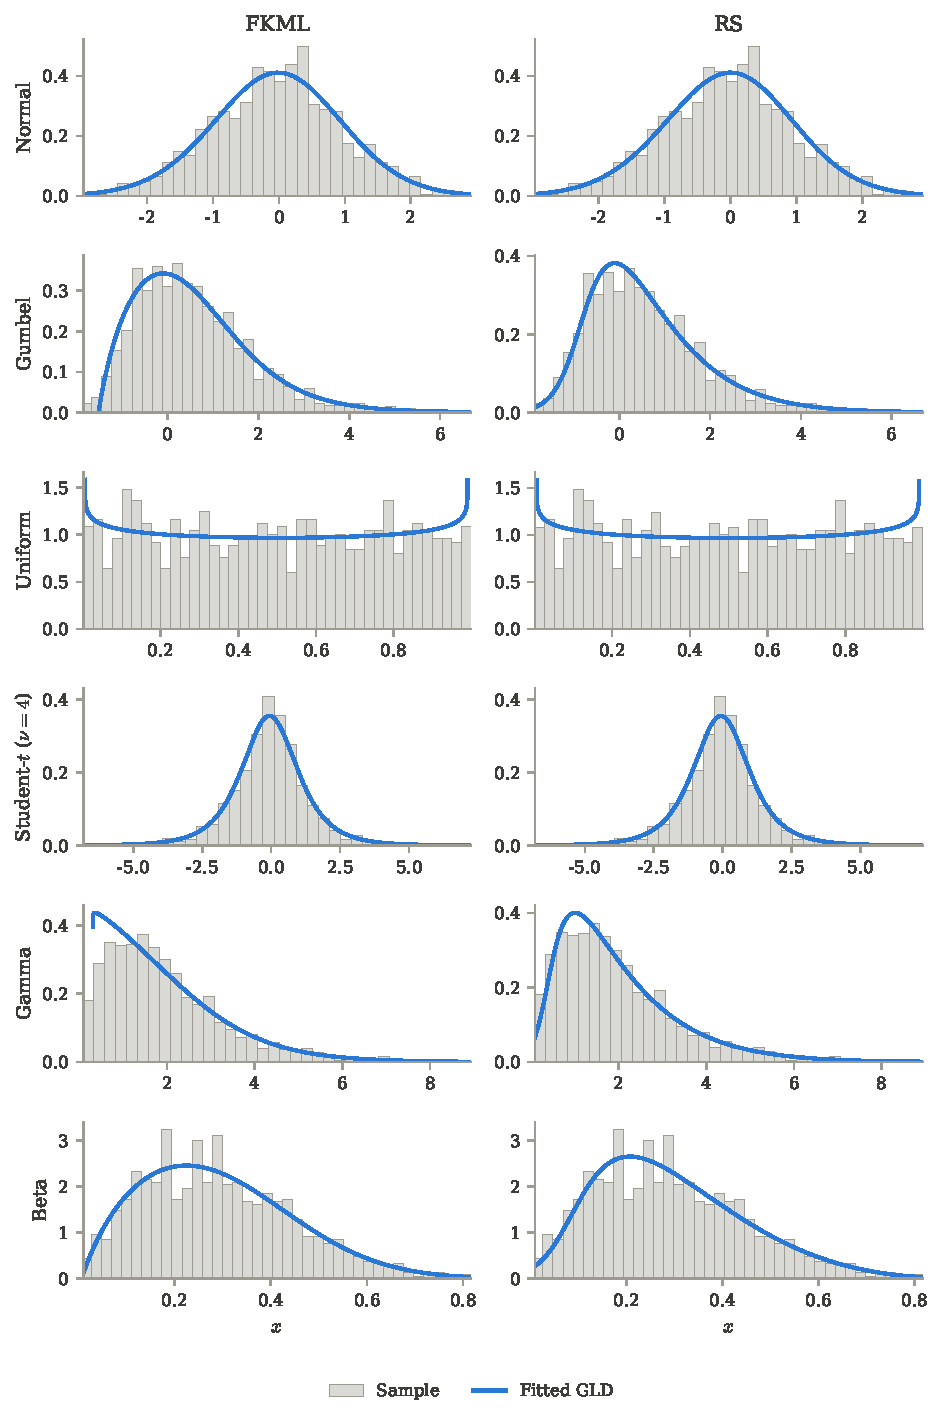
\includegraphics[width=\linewidth,height=0.86\textheight,keepaspectratio]{z_pyglam_fits_en.pdf}
    \caption{GLD fitted by moment matching to the six target distributions
    ($N = 1{,}000$), one row per target and one column per parameterization,
    both fitted to the same sample. The histogram is the sample and the solid line
    the density of the fitted GLD.}
    \label{fig:pyglam_fits}
\end{figure}

\begin{table}[p]
\centering
\caption{Fit quality of the FKML parameterization: medians over 100 independent
replicates per cell, and the interquartile range of the KS distance. Quantile
errors are normalised by the distance between the $P_5$ and the $P_{95}$ of the
target.}
\label{tab:metrics_fkml}
\small
\setlength{\tabcolsep}{4.5pt}
\begin{tabular}{lrrrrrrrr}
\toprule
\textbf{Distribution} & \textbf{$N$} & \textbf{KS} & \textbf{IQR} & \textbf{$D(p\|q)$} &
\textbf{Wass.} & \textbf{$P_5$ (\%)} & \textbf{$P_{50}$ (\%)} & \textbf{$P_{95}$ (\%)} \\
\midrule
Normal & 50 & 0.0562 & 0.0408 & 0.0651 & 0.1307 & 4.48 & 3.14 & 4.74 \\
 & 200 & 0.0320 & 0.0209 & 0.0127 & 0.0742 & 2.84 & 1.54 & 2.57 \\
 & 1,000 & 0.0137 & 0.0086 & 0.0029 & 0.0334 & 0.98 & 0.68 & 1.10 \\
 & 5,000 & 0.0067 & 0.0049 & 0.0015 & 0.0196 & 0.46 & 0.32 & 0.49 \\
\midrule
Gumbel & 50 & 0.0758 & 0.0334 & 0.1196 & 0.2019 & 3.52 & 3.48 & 7.99 \\
 & 200 & 0.0458 & 0.0314 & 0.0482 & 0.0992 & 2.09 & 1.76 & 4.46 \\
 & 1,000 & 0.0220 & 0.0128 & 0.0161 & 0.0512 & 0.87 & 0.73 & 1.91 \\
 & 5,000 & 0.0146 & 0.0059 & 0.0113 & 0.0375 & 0.41 & 0.31 & 0.98 \\
\midrule
Uniform & 50 & 0.0586 & 0.0403 & 0.0132 & 0.0320 & 2.38 & 4.07 & 2.15 \\
 & 200 & 0.0322 & 0.0217 & 0.0043 & 0.0181 & 1.11 & 2.36 & 1.05 \\
 & 1,000 & 0.0172 & 0.0114 & 0.0012 & 0.0102 & 0.54 & 1.21 & 0.61 \\
 & 5,000 & 0.0070 & 0.0033 & 0.0003 & 0.0046 & 0.20 & 0.44 & 0.21 \\
\midrule
Student-$t$ ($\nu=4$) & 50 & 0.0663 & 0.0545 & 0.2102 & 0.2328 & 7.55 & 2.68 & 6.46 \\
 & 200 & 0.0399 & 0.0287 & 0.0392 & 0.1360 & 3.55 & 1.63 & 4.51 \\
 & 1,000 & 0.0193 & 0.0125 & 0.0120 & 0.0750 & 1.73 & 0.93 & 2.33 \\
 & 5,000 & 0.0111 & 0.0073 & 0.0070 & 0.0439 & 1.07 & 0.41 & 1.11 \\
\midrule
Gamma & 50 & 0.0777 & 0.0438 & 0.0630 & 0.2150 & 2.32 & 3.43 & 10.06 \\
 & 200 & 0.0593 & 0.0285 & 0.0241 & 0.1181 & 2.14 & 2.20 & 4.44 \\
 & 1,000 & 0.0374 & 0.0194 & 0.0085 & 0.0605 & 1.44 & 1.09 & 2.37 \\
 & 5,000 & 0.0335 & 0.0122 & 0.0049 & 0.0399 & 1.21 & 0.44 & 0.94 \\
\midrule
Beta & 50 & 0.0679 & 0.0332 & 0.0452 & 0.0221 & 2.64 & 3.85 & 6.71 \\
 & 200 & 0.0329 & 0.0265 & 0.0090 & 0.0120 & 1.22 & 1.85 & 2.87 \\
 & 1,000 & 0.0180 & 0.0106 & 0.0031 & 0.0052 & 0.55 & 1.00 & 1.58 \\
 & 5,000 & 0.0095 & 0.0045 & 0.0014 & 0.0033 & 0.28 & 0.41 & 0.66
\unskip \\
\bottomrule
\end{tabular}
\end{table}

\begin{table}[p]
\centering
\caption{Fit quality of the Ramberg-Schmeiser parameterization, on the same
samples and with the same summaries as Table~\ref{tab:metrics_fkml}.}
\label{tab:metrics_rs}
\small
\setlength{\tabcolsep}{4.5pt}
\begin{tabular}{lrrrrrrrr}
\toprule
\textbf{Distribution} & \textbf{$N$} & \textbf{KS} & \textbf{IQR} & \textbf{$D(p\|q)$} &
\textbf{Wass.} & \textbf{$P_5$ (\%)} & \textbf{$P_{50}$ (\%)} & \textbf{$P_{95}$ (\%)} \\
\midrule
Normal & 50 & 0.0614 & 0.0397 & 0.0398 & 0.1334 & 5.04 & 3.23 & 4.98 \\
 & 200 & 0.0338 & 0.0208 & 0.0110 & 0.0755 & 3.29 & 1.63 & 2.81 \\
 & 1,000 & 0.0143 & 0.0083 & 0.0029 & 0.0346 & 1.06 & 0.66 & 1.01 \\
 & 5,000 & 0.0068 & 0.0052 & 0.0015 & 0.0198 & 0.52 & 0.38 & 0.54 \\
\midrule
Gumbel & 50 & 0.0682 & 0.0346 & 0.0992 & 0.1943 & 2.82 & 3.19 & 8.18 \\
 & 200 & 0.0403 & 0.0287 & 0.0195 & 0.1006 & 1.98 & 1.76 & 4.57 \\
 & 1,000 & 0.0190 & 0.0133 & 0.0052 & 0.0535 & 0.88 & 0.77 & 1.96 \\
 & 5,000 & 0.0122 & 0.0068 & 0.0029 & 0.0341 & 0.68 & 0.41 & 1.32 \\
\midrule
Uniform & 50 & 0.0592 & 0.0392 & 0.0135 & 0.0321 & 2.48 & 4.07 & 2.14 \\
 & 200 & 0.0333 & 0.0227 & 0.0044 & 0.0180 & 1.07 & 2.38 & 1.11 \\
 & 1,000 & 0.0174 & 0.0114 & 0.0013 & 0.0101 & 0.55 & 1.21 & 0.61 \\
 & 5,000 & 0.0070 & 0.0032 & 0.0003 & 0.0046 & 0.21 & 0.42 & 0.21 \\
\midrule
Student-$t$ ($\nu=4$) & 50 & 0.0666 & 0.0559 & 0.1297 & 0.2293 & 7.20 & 2.66 & 6.89 \\
 & 200 & 0.0416 & 0.0300 & 0.0328 & 0.1385 & 4.13 & 1.81 & 4.72 \\
 & 1,000 & 0.0203 & 0.0138 & 0.0117 & 0.0779 & 2.16 & 1.08 & 2.60 \\
 & 5,000 & 0.0131 & 0.0096 & 0.0070 & 0.0466 & 1.32 & 0.52 & 1.27 \\
\midrule
Gamma & 50 & 0.0742 & 0.0432 & 0.0964 & 0.2142 & 2.26 & 2.90 & 10.72 \\
 & 200 & 0.0406 & 0.0200 & 0.0328 & 0.1098 & 1.18 & 1.78 & 5.56 \\
 & 1,000 & 0.0297 & 0.0153 & 0.0251 & 0.0821 & 0.72 & 1.26 & 2.70 \\
 & 5,000 & 0.0261 & 0.0066 & 0.0292 & 0.0858 & 0.62 & 1.45 & 2.51 \\
\midrule
Beta & 50 & 0.0679 & 0.0385 & 0.0411 & 0.0224 & 2.65 & 3.62 & 6.24 \\
 & 200 & 0.0330 & 0.0230 & 0.0112 & 0.0118 & 1.33 & 1.80 & 2.42 \\
 & 1,000 & 0.0185 & 0.0110 & 0.0048 & 0.0059 & 0.88 & 0.92 & 1.35 \\
 & 5,000 & 0.0122 & 0.0056 & 0.0026 & 0.0038 & 0.69 & 0.46 & 0.78
\unskip \\
\bottomrule
\end{tabular}
\end{table}

Both parameterizations recover all six targets to a practically useful accuracy.
At $N = 5{,}000$ the median error at $P_{50}$ is at most $0.44\%$ of the
reference spread under FKML and at most $0.52\%$ under RS on every target but
the Gamma, where it is $1.45\%$; the largest median error anywhere in that row is
$2.51\%$, at the $P_{95}$ of the Gamma under RS. The coefficient of determination
between the estimated densities at $N = 5{,}000$ is at least $0.974$ for every
target except the uniform. There the fitted GLD density turns upward near the two
endpoints while the target is flat, and that comparison is also the one most
affected by the boundary bias of the kernel density estimates; the coefficient
is negative at $N = 50$ and recovers to $0.93$ at $N = 5{,}000$ under both
forms.

On the normal and the uniform the two parameterizations are practically
indistinguishable in every metric. On the Student-$t$ and the Beta, FKML reaches
the smaller KS distance at every $N \geq 1{,}000$. On the Gumbel, RS reaches the
smaller KS distance and divergence at $N = 5{,}000$. On the Gamma the ranking
depends on the metric: RS reaches the smaller KS distance at every
$N \geq 200$, and FKML the smaller divergence, Wasserstein distance and median
error at every $N \geq 1{,}000$.

\subsection{Sampling error or structural error?}\label{subsec:regimes}

The interesting question is not how large the error is but what limits it. The
error of a moment-based fit can be decomposed into a \emph{sampling} component,
from estimating four moments on a finite sample, and a \emph{structural}
component, from the family not containing the target exactly. In simplified form,
\begin{equation}
    E(N) \approx E_{\mathrm{sampling}}(N) + E_{\mathrm{structural}},
    \qquad
    E_{\mathrm{sampling}}(N) \propto N^{-1/2}.
    \label{eq:decomposition}
\end{equation}
The sampling component decreases with $N$, whereas the structural component
remains approximately constant. When the error is dominated by sampling,
\begin{equation}
    \mathrm{KS} \propto N^{-1/2}
    \quad \Longrightarrow \quad
    \log \mathrm{KS} \approx C - \tfrac{1}{2}\log N,
\end{equation}
so regressing the logarithm of the median KS distance on $\log N$ separates the
two regimes. A slope near $-1/2$ with a high coefficient of determination means
the error is predominantly sampling and the fit is as good as the data allows,
whereas a slope near zero means a structural floor dominates and more data will
not help. We label a slope below $-0.45$ as \emph{sampling-limited}, a slope
between $-0.45$ and $-0.30$ as \emph{mixed}, and a flatter one as
\emph{structural floor}. The $95\%$ confidence interval of each slope comes from
$2{,}000$ bootstrap resamples, drawn independently within each sample size.
Table~\ref{tab:rates} reports the regression and
Figure~\ref{fig:pyglam_convergence} shows it.

\begin{table}[htbp]
\centering
\caption{Convergence of the median Kolmogorov-Smirnov distance to the analytical
target: slope of $\log \mathrm{KS}$ against $\log N$ with its bootstrap $95\%$
confidence interval, coefficient of determination, and the regime the slope
implies.}
\label{tab:rates}
\small
\begin{tabular}{llrcrl}
\toprule
\textbf{Param.} & \textbf{Distribution} & \textbf{Slope} & \textbf{95\% CI} &
\textbf{$R^2$} & \textbf{Regime} \\
\midrule
FKML & Normal & $-0.467$ & $[-0.516, -0.436]$ & $0.998$ & sampling-limited \\
 & Gumbel & $-0.367$ & $[-0.387, -0.344]$ & $0.988$ & mixed \\
 & Uniform & $-0.455$ & $[-0.495, -0.409]$ & $0.993$ & sampling-limited \\
 & Student-$t$ ($\nu=4$) & $-0.396$ & $[-0.425, -0.362]$ & $0.997$ & mixed \\
 & Gamma & $-0.193$ & $[-0.228, -0.174]$ & $0.952$ & structural floor \\
 & Beta & $-0.421$ & $[-0.448, -0.394]$ & $0.995$ & mixed \\
RS & Normal & $-0.484$ & $[-0.522, -0.434]$ & $0.999$ & sampling-limited \\
 & Gumbel & $-0.383$ & $[-0.410, -0.354]$ & $0.990$ & mixed \\
 & Uniform & $-0.459$ & $[-0.499, -0.413]$ & $0.993$ & sampling-limited \\
 & Student-$t$ ($\nu=4$) & $-0.363$ & $[-0.400, -0.326]$ & $0.992$ & mixed \\
 & Gamma & $-0.221$ & $[-0.239, -0.192]$ & $0.893$ & structural floor \\
 & Beta & $-0.369$ & $[-0.392, -0.338]$ & $0.977$ & mixed
\unskip \\
\bottomrule
\end{tabular}
\end{table}

\begin{figure}[p]
    \centering
    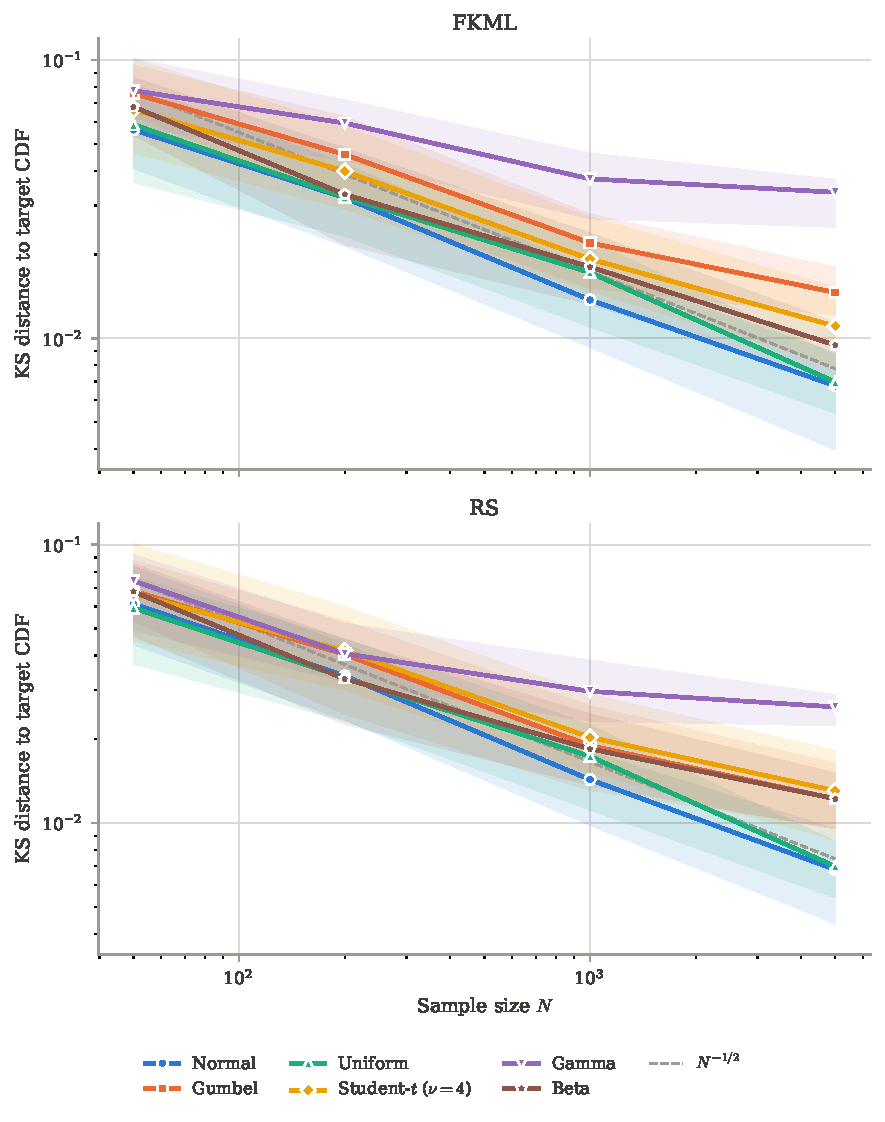
\includegraphics[width=\linewidth,height=0.86\textheight,keepaspectratio]{z_pyglam_convergence_en.pdf}
    \caption{Convergence of the Kolmogorov-Smirnov distance between the fitted
    GLD and the analytical target, against sample size, one panel per
    parameterization. Logarithmic axes; each point is the median of 100
    independent replicates and the band their interquartile range. The dashed
    guide has slope $-1/2$, the theoretical sampling rate.}
    \label{fig:pyglam_convergence}
\end{figure}

For the normal and the uniform the two parameterizations behave identically and
converge close to the theoretical rate, with slopes between $-0.484$ and $-0.455$
and $R^2 \geq 0.993$. There is no detectable structural component: the GLD
represents a symmetric unbounded target and a bounded one with the precision the
data allows, and the choice of parameterization is immaterial.

The Beta and the Gumbel fall in the mixed regime under both forms, a small
structural component that slows the decay without stopping it. On the Gumbel the
two confidence intervals overlap, $[-0.387, -0.344]$ under FKML and
$[-0.410, -0.354]$ under RS, and the rates cannot be told apart. The fitted
parameters show that the two forms reach the exponential right tail of the
Gumbel in different ways. In the FKML form an exponential tail is the
logarithmic case $\lambda_4 = 0$ of Equation~\eqref{eq:qfkml}, and the fits
settle near it, at a median $\lambda_4 = -0.024$ at $N = 5{,}000$. The RS form
has no logarithmic case: it can only approach an exponential tail as the limit
in which $\lambda_2$, $\lambda_3$ and $\lambda_4$ vanish together while their
ratios stay finite, and that is where its fits go, with all three medians within
$0.04$ of zero. The limit is the common edge of the region with positive shapes
and the region with negative shapes, and the fits land on both sides of it: at
$N = 5{,}000$, $14\%$ of them have $\lambda_2 < 0$, with a median KS distance of
$0.0178$ against $0.0119$ for the others.

The Gamma is the one target with a structural floor under both forms, with
slopes of $-0.193$ (FKML) and $-0.221$ (RS). Its density rises linearly from zero
at the left endpoint, which neither moment-matched GLD reproduces. The FKML fit,
at a median $\lambda_3 = 0.94$ and $\lambda_4 = -0.005$, rises almost vertically
at that endpoint (Figure~\ref{fig:pyglam_fits}), and its median KS distance stops
at $0.034$. The RS fit takes a strongly asymmetric shape, with a median
$\lambda_3 = 31$ and $\lambda_4 = 0.63$, whose density at the left endpoint is
finite and positive; its median KS distance stops at $0.026$, at the price of
the larger divergence and median error noted above. Both fits reproduce the same
four sample moments, and they differ in which part of the distribution they get
wrong, which is the case for scoring every fit with the diagnostics of
Section~\ref{sec:software} rather than trusting the moment match alone.

The Student-$t$ shows a mixed regime under both forms, with slopes of $-0.396$
under FKML and $-0.363$ under RS. Here the limitation is not the family but the
estimator. Because the kurtosis of the target is infinite, the sample kurtosis
does not converge: over the replicates of the study its median grows from $4.1$
at $N = 50$ to $10.2$ at $N = 5{,}000$. The moments being matched therefore move
with $N$, and the fitted shapes follow them towards the pole of the fourth
moment: the median $\lambda_3$ goes from $-0.02$ at $N = 200$ to $-0.14$ at
$N = 5{,}000$ under FKML, and from $-0.06$ to $-0.14$ under RS. With both shapes negative the fitted
distributions are unbounded on both sides, as the target is, but moment matching
cannot settle on a limit, and the convergence slows accordingly.

Three consequences follow. First, whether a structural component appears depends
on the target: none for the normal and the uniform, a small one for the Gumbel
and the Beta, a floor for the Gamma. Second, where the parameterizations differ,
the difference is not always in the rate but in the shape of the error: on the
Gamma the two forms match the same moments with distributions that fail in
different places, and on the Gumbel a share of the RS fits falls on the wrong
side of a degenerate limit, which a study of one parameterization, or of mean errors
alone, would not reveal. Third, the regime decomposition also diagnoses
the estimator, as the Student-$t$ shows: a target at the edge of the moment
domain slows moment matching under either form, and the remedy there is a
different estimator rather than a different parameterization.

The classical test behaves as its power dictates. At the $5\%$ level, the
rejection rate of the Kolmogorov-Smirnov test at size $N$ stays between $3\%$ and
$9\%$ for the normal at every sample size, consistent with the nominal level. On
the targets with a structural component it grows with $N$ while the fit itself
improves: at $N = 5{,}000$ it reaches $26\%$ (FKML) and $35\%$ (RS) on the Gumbel,
$24\%$ and $29\%$ on the Student-$t$, and $76\%$ and $74\%$ on the Gamma. The
apparent paradox is only the test gaining power: with more data it detects a
residual discrepancy that remains small in magnitude.

\subsection{Validity and cost of the fits}\label{subsec:validity_results}

Section~\ref{subsec:validity} showed that validity is a sign condition on
$\lambda_2$ under FKML and a region condition under RS, and
Section~\ref{sec:software} described how the estimator enforces both.
Table~\ref{tab:validity} reports the result, together with the fitting time.

\begin{table}[htbp]
\centering
\caption{Validity and cost of the fits, over 400 fits per cell.
\emph{Candidates} is the share of the 15 multi-start candidates whose quantile
function is finite and non-decreasing; \emph{selected} is the share of the fits
returned by the estimator that are distributions. The optimizer reported
convergence for every fit. Times are per fit, in seconds.}
\label{tab:validity}
\small
\begin{tabular}{llrrrrr}
\toprule
& & & \multicolumn{2}{c}{\textbf{Valid (\%)}} & \multicolumn{2}{c}{\textbf{Time (s)}} \\
\cmidrule(lr){4-5} \cmidrule(lr){6-7}
\textbf{Param.} & \textbf{Distribution} & \textbf{Fits} &
\textbf{Candidates} & \textbf{Selected} & \textbf{Mean} & \textbf{SD} \\
\midrule
FKML & Normal & 400 & 100.0 & 100.0 & 0.19 & 0.34 \\
 & Gumbel & 400 & 100.0 & 100.0 & 0.16 & 0.11 \\
 & Uniform & 400 & 99.6 & 100.0 & 2.29 & 2.01 \\
 & Student-$t$ ($\nu=4$) & 400 & 100.0 & 100.0 & 0.20 & 0.13 \\
 & Gamma & 400 & 100.0 & 100.0 & 0.33 & 0.44 \\
 & Beta & 400 & 100.0 & 100.0 & 0.26 & 0.58 \\
RS & Normal & 400 & 100.0 & 100.0 & 0.20 & 0.11 \\
 & Gumbel & 400 & 100.0 & 100.0 & 0.30 & 0.14 \\
 & Uniform & 400 & 100.0 & 100.0 & 0.26 & 0.12 \\
 & Student-$t$ ($\nu=4$) & 400 & 100.0 & 100.0 & 0.28 & 0.14 \\
 & Gamma & 400 & 100.0 & 100.0 & 0.30 & 0.13 \\
 & Beta & 400 & 100.0 & 100.0 & 0.32 & 0.22
\unskip \\
\bottomrule
\end{tabular}
\end{table}

Every selected fit is a distribution. Under RS every candidate is one as well,
because the admissible regions are imposed inside the residual function and the
solver never leaves them. Under FKML the objective does not constrain the sign of
$\lambda_2$, and $29$ of the $36{,}000$ candidates were not distributions, $28$ of
them because they ended with $\lambda_2 < 0$: parameter vectors that reproduce
the four sample moments and are reported as converged by the optimizer, yet whose
quantile function is decreasing. Most of them, $24$, occur on the uniform. The
screens of
Section~\ref{sec:software} exclude them before selection. The general point is
that optimizer convergence says nothing about validity: the moment equations
admit such roots, and only an explicit check keeps them out of the result.

A fit takes $0.28$ seconds on average under RS, with little dispersion, and
$0.57$ seconds under FKML, with a median of $0.18$ seconds and a long right tail
driven by the uniform target, where a fit takes $2.29$ seconds on average. These
times were measured inside $31$ worker processes running in parallel on a
$32$-thread workstation, and the whole study, including the scoring of every
fit, took about seven minutes of wall time.

\subsection{Comparison with the R implementations}\label{subsec:r_comparison}

The implementation was cross-validated against the R packages \texttt{gld}
\parencite{KingGld} and \texttt{GLDEX} \parencite{Su2007JSS, SuGLDEX}, running on
R 4.6.1 \parencite{RCore}, in two parts.

The first part compares the functions themselves. For six parameter vectors of
each parameterization, spanning the fits of this study, asymmetric and
heavy-tailed shapes, and, for RS, the regions with positive, negative and mixed
signs, the quantile function, the CDF and the density of \texttt{pyGLAM} were
evaluated on $199$ probabilities and compared with \texttt{qgl}, \texttt{pgl} and
\texttt{dgl} of \texttt{gld}, and the first four moments with
\texttt{fun.theo.mv.gld} of \texttt{GLDEX}. Table~\ref{tab:r_functions} reports
the largest discrepancy. The quantile functions agree to rounding error and the
moments to $10^{-9}$ or better; the CDF and the density agree to $10^{-8}$, the
tolerance of the numerical inversion of the quantile function.

\begin{table}[htbp]
\centering
\caption{Largest discrepancy between \texttt{pyGLAM} and the R packages over six
parameter vectors per parameterization: quantile relative to the range of the
evaluated quantiles, CDF in probability, density relative to its maximum, mean in
standard deviations, variance relatively, skewness and kurtosis in absolute
terms.}
\label{tab:r_functions}
\footnotesize
\setlength{\tabcolsep}{3.5pt}
\begin{tabular}{lrccccccc}
\toprule
\textbf{Param.} & \textbf{Sets} & \textbf{Quantile} & \textbf{CDF} & \textbf{Density} &
\textbf{Mean} & \textbf{Variance} & \textbf{Skewness} & \textbf{Kurtosis} \\
\midrule
FKML & 6 & $2.0 \times 10^{-15}$ & $1.0 \times 10^{-8}$ & $1.2 \times 10^{-8}$ & $5.4 \times 10^{-16}$ & $5.7 \times 10^{-15}$ & $7.1 \times 10^{-14}$ & $1.5 \times 10^{-12}$ \\
RS & 6 & $1.4 \times 10^{-15}$ & $1.0 \times 10^{-8}$ & $1.5 \times 10^{-8}$ & $2.3 \times 10^{-15}$ & $8.0 \times 10^{-15}$ & $2.0 \times 10^{-13}$ & $5.1 \times 10^{-10}$
\unskip \\
\bottomrule
\end{tabular}
\end{table}

The second part compares the fits. Fifty samples of each target at
$N = 1{,}000$ and $N = 5{,}000$ were fitted by moment matching with
\texttt{pyGLAM} and with \texttt{fun.RMFMKL.mm} and \texttt{fun.RPRS.mm} of
\texttt{GLDEX}, and every fit was scored by the same code. Because the moment
equations have several roots, the parameters are not expected to coincide; the
comparison is on the fitted distributions, and Table~\ref{tab:r_fits} reports
the KS distance and the Wasserstein distance to the analytical target, the
latter normalised by the distance between the $P_5$ and the $P_{95}$ of the
target, together with the largest gap between the two fitted quantile functions
on $[0.01, 0.99]$, in the same units. All $2{,}400$ fits of both packages were
valid distributions.

\begin{table}[htbp]
\centering
\caption{Fits of the same samples by \texttt{pyGLAM} (py) and \texttt{GLDEX} (R):
share of valid fits, medians over 50 samples of the KS distance and of the
normalised Wasserstein distance to the target, and median of the largest gap
between the two fitted quantile functions.}
\label{tab:r_fits}
\footnotesize
\setlength{\tabcolsep}{3.5pt}
\begin{tabular}{llrrrrrrrr}
\toprule
& & & \multicolumn{2}{c}{\textbf{Valid (\%)}} & \multicolumn{2}{c}{\textbf{KS}} &
\multicolumn{2}{c}{\textbf{Wasserstein}} & \textbf{Quantile} \\
\cmidrule(lr){4-5} \cmidrule(lr){6-7} \cmidrule(lr){8-9}
\textbf{Param.} & \textbf{Distribution} & \textbf{$N$} & \textbf{py} & \textbf{R} &
\textbf{py} & \textbf{R} & \textbf{py} & \textbf{R} & \textbf{gap} \\
\midrule
FKML & Normal & 1,000 & 100 & 100 & 0.0124 & 0.0124 & 0.0090 & 0.0090 & 0.0000 \\
 &  & 5,000 & 100 & 100 & 0.0057 & 0.0057 & 0.0041 & 0.0041 & 0.0000 \\
 & Gumbel & 1,000 & 100 & 100 & 0.0261 & 0.0230 & 0.0154 & 0.0143 & 0.0609 \\
 &  & 5,000 & 100 & 100 & 0.0146 & 0.0187 & 0.0078 & 0.0099 & 0.0640 \\
 & Uniform & 1,000 & 100 & 100 & 0.0142 & 0.0150 & 0.0086 & 0.0100 & 0.0036 \\
 &  & 5,000 & 100 & 100 & 0.0067 & 0.0076 & 0.0037 & 0.0043 & 0.0021 \\
 & Student-$t$ ($\nu=4$) & 1,000 & 100 & 100 & 0.0180 & 0.0180 & 0.0148 & 0.0148 & 0.0000 \\
 &  & 5,000 & 100 & 100 & 0.0101 & 0.0101 & 0.0090 & 0.0090 & 0.0000 \\
 & Gamma & 1,000 & 100 & 100 & 0.0413 & 0.0250 & 0.0141 & 0.0131 & 0.0516 \\
 &  & 5,000 & 100 & 100 & 0.0313 & 0.0243 & 0.0083 & 0.0098 & 0.0461 \\
 & Beta & 1,000 & 100 & 100 & 0.0171 & 0.0290 & 0.0100 & 0.0187 & 0.0413 \\
 &  & 5,000 & 100 & 100 & 0.0096 & 0.0283 & 0.0048 & 0.0173 & 0.0422 \\
\midrule
RS & Normal & 1,000 & 100 & 100 & 0.0138 & 0.0138 & 0.0094 & 0.0094 & 0.0000 \\
 &  & 5,000 & 100 & 100 & 0.0060 & 0.0060 & 0.0040 & 0.0040 & 0.0000 \\
 & Gumbel & 1,000 & 100 & 100 & 0.0200 & 0.0302 & 0.0135 & 0.0197 & 0.0443 \\
 &  & 5,000 & 100 & 100 & 0.0110 & 0.0121 & 0.0063 & 0.0068 & 0.0000 \\
 & Uniform & 1,000 & 100 & 100 & 0.0144 & 0.0149 & 0.0086 & 0.0097 & 0.0038 \\
 &  & 5,000 & 100 & 100 & 0.0067 & 0.0076 & 0.0037 & 0.0047 & 0.0024 \\
 & Student-$t$ ($\nu=4$) & 1,000 & 100 & 100 & 0.0195 & 0.0272 & 0.0160 & 0.0190 & 0.0000 \\
 &  & 5,000 & 100 & 100 & 0.0122 & 0.0122 & 0.0101 & 0.0101 & 0.0000 \\
 & Gamma & 1,000 & 100 & 100 & 0.0292 & 0.0252 & 0.0192 & 0.0147 & 0.1197 \\
 &  & 5,000 & 100 & 100 & 0.0275 & 0.0153 & 0.0192 & 0.0083 & 0.1238 \\
 & Beta & 1,000 & 100 & 100 & 0.0176 & 0.0180 & 0.0109 & 0.0113 & 0.0000 \\
 &  & 5,000 & 100 & 100 & 0.0111 & 0.0124 & 0.0062 & 0.0071 & 0.0000
\unskip \\
\bottomrule
\end{tabular}
\end{table}

On the normal and the Student-$t$ the two packages return the same distribution
under both parameterizations, with a quantile gap below $10^{-4}$, and so they
do for the RS fits of the Beta and, at $N = 5{,}000$, of the Gumbel. On the
uniform the gaps stay below $0.004$. Elsewhere the two packages land on different
solutions, for two different reasons. Under FKML, \texttt{pyGLAM} reproduces the
sample moments to the precision of the solver, whereas \texttt{GLDEX} stops at a
median moment discrepancy of $0.08$ to $0.10$ on the Gumbel, the Gamma and the
Beta. The inexact solution is not always the worse one: it is farther from the
target on the Beta, with a median KS distance of $0.028$ against $0.010$ at
$N = 5{,}000$, but closer on the Gamma, with $0.024$ against $0.031$, another
instance of a closer moment match not being a closer distribution. Under RS,
both packages reproduce the moments of the Gamma, but at different roots: the
dense search of \texttt{GLDEX}, over $10{,}000$ quasi-random starting points,
reaches one with a median KS distance of $0.015$, whereas the $15$ starts of
\texttt{pyGLAM} reach $0.027$, and the full grid of $29$ starts $0.025$.

\texttt{pyGLAM} is also faster. Measured under the same conditions, with one
process per core, a fit takes a median of $0.17$ seconds under FKML and $0.18$
under RS, against $1.09$ and $4.92$ seconds for \texttt{GLDEX}.

\section{Concluding remarks}\label{sec:conclusions}

This paper introduced \texttt{pyGLAM}, a Python package implementing the FKML and
Ramberg-Schmeiser parameterizations of the generalized lambda distribution behind
one interface, fitting them by multi-start moment matching and scoring the result
with an integrated goodness-of-fit module. A cross-validation against the R
packages and a factorial Monte Carlo study over two parameterizations, six
targets, four sample sizes and one hundred replicates per cell established four
things.

First, the implementation agrees with \texttt{gld} and \texttt{GLDEX}: the
quantile functions, distribution functions, densities and moments coincide to
numerical precision, and on the same samples the fits of \texttt{pyGLAM} are
valid, reproduce the sample moments, and take a fraction of the time. Where the
two packages reach different fits, the difference comes from how they solve the
moment equations and which root they reach, not from the functions they
evaluate.

Second, moment matching recovers all six targets to a practically useful
accuracy: at $N = 5{,}000$ the median error at $P_{50}$ is below $0.5\%$ of the
spread between $P_5$ and $P_{95}$ in ten of the twelve cases, at a mean cost of
well under a second per fit.

Third, the error separates into a sampling component and a structural one, and
the slope of the Kolmogorov-Smirnov distance against sample size tells them
apart. The normal and the uniform show no structural component under either
parameterization, the Gumbel and the Beta a small one, and the Gamma a floor
under both. On the Gamma the two parameterizations match the same moments with
distributions that fail in different places, so which one is better depends on
the metric that scores them; on the Gumbel the RS fits approach the exponential
tail through a degenerate limit of their parameters that the FKML form contains
as a regular case. On the Student-$t$ with four degrees of freedom both forms
slow down because the kurtosis of the target is infinite, which makes the
decomposition a diagnostic of the estimator as well. Since the Python
implementations we are aware of commit to a single parameterization, a
practitioner using them accepts whatever structural component that form carries
on their target, without being told. This is the argument for carrying more than
one form, and a diagnostic, in the same package.

Fourth, four-moment matching admits roots that reproduce the four sample moments,
are reported as converged by the optimizer, and are not distributions. Imposing
the admissible regions inside the RS objective, starting the multi-start on both
sides of those regions, and screening the candidates of both forms for a
non-decreasing quantile function kept every one of the $4{,}800$ selected fits
valid.

Several limitations point to the next steps. The package currently offers one
estimator, and moment matching is known to be the weakest of the GLD estimators;
the Student-$t$ case shows its limits directly. L-moments
\parencite{KarvanenNuutinen2008}, which exist whenever the mean does, percentile
matching \parencite{KarianDudewicz1999} and discretised maximum likelihood
\parencite{Su2007CSDA} are the natural additions, and the regime decomposition
used here transfers directly to comparing them. The comparison with
\texttt{GLDEX} shows that a denser search of starting points can reach better
roots of the RS moment equations on some targets, at a much higher cost; an
adaptive search that spends more starts only where the candidates disagree would
combine the two. The study covers six targets, chosen for geometric contrast;
multimodal targets, which a single GLD cannot represent, call for mixtures. The
\texttt{cdf} and \texttt{pdf} methods invert the quantile function elementwise
and would benefit from a vectorised inversion.


\section*{Author contributions}
Author contributions follow the CRediT taxonomy.
\textbf{Wanderlei Malaquias Pereira Junior:} Methodology, Validation,
Supervision, Writing -- original draft, Writing -- review \& editing.
\textbf{Marcos Luiz Henrique:} Methodology, Formal analysis, Validation.
\textbf{Ketson Roberto Maximiano dos Santos:} Methodology, Supervision,
Writing -- original draft, Writing -- review \& editing.
\textbf{Victor Hugo Moreira do Couto Souza:} Methodology, Validation,
Visualization, Writing -- original draft, Writing -- review \& editing.
\textbf{Renata Maria Pensin:} Validation, Visualization.

\section*{Acknowledgements and funding}
The authors thank the Funda\c{c}\~ao de Amparo \`a Pesquisa do Estado de
Goi\'as (FAPEG) for the scholarship granted to Victor Hugo Moreira do Couto
Souza.

\printbibliography

\end{document}
